%% Direttive TeXworks:
% !TeX root = ../semprini_luca_tesi.tex
% !TEX encoding = UTF-8 Unicode
% !TEX program = arara
% !TEX TS-program = arara
% !TeX spellcheck = it-IT

%% Direttive Arara:
% arara: pdflatex: { shell: yes, synctex: yes, action: batchmode, options: "-halt-on-error -file-line-error-style" }
% arara: frontespizio
% arara: biber
% arara: pdflatex: { shell: yes, synctex: yes, action: batchmode, options: "-halt-on-error -file-line-error-style" }
% arara: pdflatex: { shell: yes, synctex: yes, action: nonstopmode, options: "-halt-on-error -file-line-error-style" }

\chapter{La sintassi di Kotlin}\label{ch:sintassi}
Come accennato nel capitolo precedente, la sintassi di Kotlin è destinata ad essere concisa, ma senza pregiudicare la leggibilità. Essa sostiene la tradizionale struttura a blocchi nidificati basata sulle parentesi graffe, ma presenta anche inferenze implicite di punti e virgola: questo significa che sarà totalmente facoltativo inserirli al termine di un'operazione. I whitespace (tranne gli a capo) sono generalmente non significativi (ad eccezione di stringhe e caratteri letterali), ma in alcuni casi sono necessari per separare alcuni token. La sintassi di Kotlin prende particolarmente spunto da quella di linguaggi come Scala, Groovy e ovviamente Java; gli sviluppatori del team diretto da Andrey Breslav hanno cercato di coniugare le peculiarità di questi linguaggi di riferimento, per creare un nuovo linguaggio JVM che potesse superarne i limiti sintattici e semantici. Il paradigma principale sul quale si fonda è quello ad oggetti, ma inserendovi caratteristiche di tipo funzionale: le funzioni possono essere, quindi, considerate come valori "first-class": hanno tipo, possono essere passate come argomenti, restituite come valori di ritorno e memorizzate in variabili locali, campi di classi ed elementi di array.\\

\section{Esempio di Hello World}
Per inquadrare la sintassi basilare del linguaggio, si riporta di seguito un esempio classico di un programma che stampi "Hello, world": in Kotlin esso consiste in una singola funzione:\\
\\

\begin{lstlisting}[caption={Hello World}, captionpos=b, label={lst:exampleHelloWorld}, language=Kotlin]
fun main(args: Array<String>) {
  println("Hello, world!")
}
\end{lstlisting}

Da questo primo snippet di codice si possono facilmente notare (e intuire) le caratteristiche sintattiche principali del linguaggio:
\begin{itemize}
  \item Viene utilizzata la parola chiave \texttt{fun} per dichiarare una funzione.
  \item Il tipo del parametro in ingresso viene scritto dopo l’identificativo, separandoli con i due punti. Questo vale anche per le dichiarazioni di variabili.
  \item Una funzione può essere dichiarata al top-level in un file Kotlin, dunque non necessariamente all’interno di una classe.
  \item Gli array sono semplicemente classi: a differenza di Java, Kotlin non dispone di una sintassi specifica per la dichiarazione di array.
  \item La stampa su standard output è definita dalla funzione println (differentemente dalla sintassi Java: \texttt{System.out.println}). La libreria standard di Kotlin fornisce molti wrapper per le funzioni della standard library Java, aggiungendo una sintassi più concisa e comprensibile e la funzione di stampa è una di esse.
  \item È possibile, come già analizzato, omettere il punto e virgola alla fine di una linea di codice.
\end{itemize}

Un’altra particolarità del linguaggio riguarda i blocchi \texttt{if-else}: non si tratta di uno statement, ma di una vera e propria espressione. La differenza sta nel fatto che una espressione ha un valore che può
essere utilizzato come parte di un'altra espressione, mentre uno statement è sempre un elemento top-level nel suo blocco, e non ha un proprio valore. Mentre in Java, tutte le strutture di controllo sono statements, qui la maggior parte di esse, ad eccezione dei loop (\texttt{for}, \texttt{do} e \texttt{do-while}) sono espressioni.
La possibilità di combinare strutture di controllo con altre espressioni consente di esprimere molti pattern comuni in maniera più potente e concisa. D'altra parte, le assegnazioni sono espressioni in Java e diventano statements in Kotlin: ciò consente di evitare la confusione tra confronti e assegnazioni, che è spesso una tipica fonte di errori.\\
In Kotlin è possibile semplificare le funzioni il cui corpo consiste in una singola espressione: rimuovendo le parentesi graffe e l'istruzione \texttt{return}, e sostituendoli con l'operatore "\texttt{=}", seguito appunto dalla singola espressione si otterrà quella che viene chiamata inline-function:

\begin{lstlisting}[caption={Inline-function}, captionpos=b, label={lst:exampleInlineFunction}, language=Kotlin]
fun max(a: Int, b: Int): Int = if (a > b) a else b
\end{lstlisting}

Questo tipo di funzioni sono chiamate, in Kotlin, anche funzioni con expression body, mentre le classiche funzioni con le parentesi graffe hanno un block body; IntelliJ IDEA fornisce una funzionalità in cui può suggerire di scambiare in maniera trasparente i due stili: "Convert to expression body", "Convert to block body".\\

Nel caso preso in esempio, è, inoltre, possibile omettere la dichiarazione del tipo di ritorno:
per funzioni di tipo expression-body, infatti, il compilatore può analizzare l'espressione usata come corpo della funzione e utilizzare il suo tipo come tipo di ritorno di funzione, anche quando non viene dichiarato in modo esplicito. Questo tipo di analisi prende tipicamente il nome di inferenza di tipo. Si noti che l'omissione del tipo di ritorno è consentita solo per funzioni con un'espressione come corpo.\\

\section{Variabili e String Templates}
La dichiarazione di una variabile, in Kotlin, viene effettuata digitando inizialmente una keyword:
\begin{itemize}
  \item {\bfseries\texttt{var}}: Riferimento immutabile. Una variabile dichiarata con val non può essere
  riassegnata dopo l'inizializzazione: corrisponde a una variabile \texttt{final} in Java. Di default, le specifiche del linguaggio invitano a cercare di dichiarare tutte le variabili in Kotlin con la parola chiave val, ed utilizzare il riferimento mutabile solo se strettamente necessario. Utilizzare riferimenti immutabili, oggetti immutabili e funzioni senza side-effect rende il codice più vicino allo stile funzionale.
  \item {\bfseries\texttt{val}}: Riferimento mutabile. Il valore di tale variabile può essere modificato: questa dichiarazione corrisponde a una normale variabile Java (non \texttt{final}).
\end{itemize}

Successivamente va digitato l'identificativo, e infine, facoltativamente, il tipo: infatti, il compilatore permette l'inferenza di tipo anche per la dichiarazione di variabili, anche se, ovviamente, il compilatore non può dedurre il tipo se non si forniscono informazioni sui valori che possono
essere assegnati a questa variabile (quindi nel caso di non specificazione del tipo, va sempre eseguito un assegnamento). Si noti, quindi, l'equivalenza delle seguenti scritture:

\begin{lstlisting}[caption={Inferenza di tipo}, captionpos=b, label={lst:exampleInferenzaDiTipo}, language=Kotlin]
val number: Int = 1 //Tipo esplicitato
val number = 1      //Il tipo viene inferito dal compilatore
\end{lstlisting}

Per quanto riguarda il sistema di tipi, in Kotlin esiste un singolo tipo di root (\texttt{kotlin.Any?}) e ogni altro tipo è suo sottotipo (si parla, quindi, di un sistema di tipi unificato): una delle grandi differenze di Kotlin rispetto a Java è che nel linguaggio progettato dal team di JetBrains tutto è un oggetto; non esistono, quindi, speciali tipi primitivi che vengono trattati in modo diverso dagli oggetti. Tuttavia, per motivi di prestazioni, quando possibile, il compilatore Kotlin mapperà questi tipi di base con quelli primitivi della JVM.\\

Nella gestione delle stringhe, Kotlin aggiunge una funzionalità che semplifica diverse situazioni: essa viene denominata "{\em String templates}". Come molti linguaggi di scripting, Kotlin permette di fare riferimento a variabili locali nelle rappresentazioni di stringhe, mettendo il carattere "\texttt{\$}" davanti al nome della variabile che si desidera chiamare (se vi è la necessità di inserire il carattere "\texttt{\$}" all’interno di una stringa è possibile utilizzare l’operatore di escape "\texttt{\textbackslash}" prima del carattere stesso). Questo equivale alla concatenazione stringhe in Java (\texttt{"Chiamata " + variabile + " in Java"}), ma risulta molto più compatto e altrettanto efficiente, inoltre, le espressioni vengono controllate staticamente e il codice non verrà compilato se si tenta di fare riferimento a una variabile che non esiste. Oltre alle semplici variabili, è possibile inserire in uno String template anche espressioni più complesse, semplicemente circondandole da parentesi graffe (questa notazione permette anche di nidificare le doppie virgolette all'interno di una rappresentazione di stringa):\\

\begin{lstlisting}[caption={String Template}, captionpos=b, label={lst:exampleStringTemplate}, language=Kotlin]
fun main(args: Array<String>) {
  println("Hello, ${if (args.size > 0) args[0] else "someone"}!")
}
\end{lstlisting}

\section{Classi e Proprietà}
Il linguaggio di JetBrains introduce importanti novità soprattutto nell’ambito dei costruttori e dei campi delle classi. In Java, il corpo del costruttore contiene spesso codice che risulta interamente ripetitivo: assegna, per esempio, i parametri ai campi con nomi corrispondenti; in Kotlin, questa logica può essere espressa senza troppo boilerplate: viene introdotta la possibilità di inserire i campi che in Java sarebbero stati rappresentati come parametri del costruttore direttamente nella dichiarazione della classe, assegnandoli direttamente ai campi corrispettivi.\\

\begin{lstlisting}[caption={Classe \texttt{Person} con una proprietà \texttt{name}}, captionpos=b, label={lst:exampleClassDeclaration}, language=Kotlin]
class Person(val name: String)
\end{lstlisting}

Le classi di questo tipo (contenenti solo dati ma nessuna riga di codice) sono spesso
chiamate "{\em value objects}", e molti linguaggi moderni offrono una sintassi sintetica per dichiararli.
Semplici classi scritte con questo stile possono risultare molto più semplici e intuitive da affrontare rispetto alla rispettiva versione Java, specie se dotate di un elevato numero di campi.\\
Si noti, inoltre, che il modificatore \texttt{public} non viene inserito, in quanto scomparso nel linguaggio Kotlin: viene omesso poiché \texttt{public} è la visibilità predefinita. Allo stesso modo, tutte le dichiarazioni di metodi all’interno di una classe sono implicitamente definite come \texttt{final}, a meno che non si aggiunga la keyword \texttt{open}, che significa che si intende esplicitamente rendere quel metodo o quella proprietà sovrascrivibile in una sottoclasse. Per sovrascrivere metodi di una sopra-classe è necessario inserire la parola chiave \texttt{override}.\\

In Java, la combinazione del campo e dei suoi metodi accessori (getter e setter) viene spesso definita come proprietà, e molti framework sfruttano e utilizzano fortemente questo concetto. In Kotlin, le proprietà sono una feature first-class del linguaggio, che sostituisce interamente i campi ed i metodi accessori: in Kotlin si dichiara una proprietà in una classe allo stesso modo in cui si dichiara una variabile, ovvero utilizzando le keyword \texttt{val} e \texttt{var}. Una proprietà dichiarata come val risulta di sola lettura (quindi corrispondente ad un campo final in Java), questa dichiarazione genera un campo e un getter corrispondenti alla proprietà; una proprietà var è mutevole e può essere cambiata, genera quindi un campo, un getter e un setter. Di default, l'implementazione degli accessori è banale: viene creato un campo per memorizzare il valore e il getter e il setter ritornano e aggiornano questo valore; tuttavia, è possibile dichiarare metodi accessori personalizzati che utilizzano logiche diverse per calcolare o aggiornare il valore della proprietà.\\

\begin{figure}[ht]
  \centering
  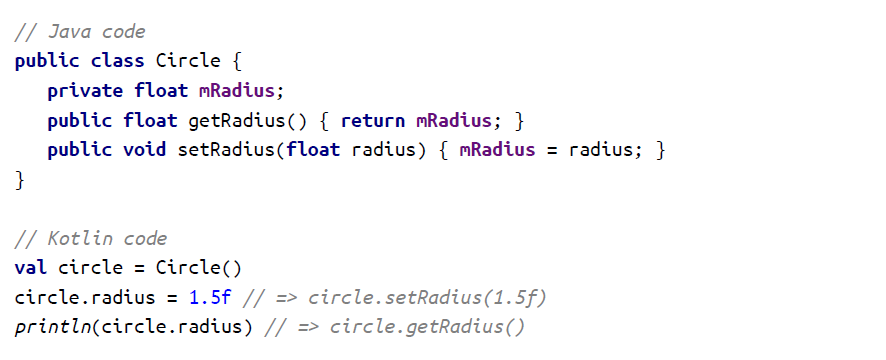
\includegraphics[scale=0.75]{Properties.png}
  \caption{{\bfseries Esempio di utilizzo delle proprietà}}
  \label{KotlinProperties}
\end{figure}

La figura \ref{KotlinProperties} rappresenta un esempio di come sia semplice la sintassi Kotlin per chiamare metodi getter e setter da classi definite in Java.\\

È inoltre possibile utilizzare questa sintassi delle proprietà di Kotlin per le classi definite in Java.\\
In particolare, getter in una classe Java sono accessibili come proprietà \texttt{val} da Kotlin, e le coppie getter/setter possono essere accedute come proprietà \texttt{var}. Ad esempio, se una classe Java definisce degli ipotetici metodi chiamati \texttt{getName()} e \texttt{setName()}, è possibile accedervi con una proprietà Kotlin denominata \texttt{name}. Se la classe Java definisce, ancora, dei metodi \texttt{isMarried()} e \texttt{setMarried()} per un ipotetico campo booleano, il nome della corrispondente proprietà Kotlin sarà \texttt{isMarried}; per cui, riprendendo l'esempio di classe generica \texttt{Person}, la sintassi delle proprietà sarà la seguente:\\

\begin{lstlisting}[caption={Utilizzo delle proprietà di una classe Kotlin}, captionpos=b, label={lst:exampleProperties}, language=Kotlin]
class Person(
  val name: String,
  var isMarried: Boolean
)

//Istanziazione

val bob = Person("Bob", true) //Oppure, in alternativa:
val bob = Person(name = "Bob", isMarried = true)  //In maniera piu' espressiva
val bob = Person(isMarried = true, name = "Bob")  //Ordine irrilevante con questa sintassi
\end{lstlisting}

Si noti, nell'esempio \ref{lst:exampleProperties}, come l'istanziazione di un oggetto nel linguaggio Kotlin non richieda l'utilizzo della keyword \texttt{new}. In Kotlin, è possibile, inoltre, definire dei valori di default da assegnare a proprietà della classe che si sta definendo, in modo da evitare la ripetizione non necessaria di codice che comporta, in Java, la scrittura di differenti costruttori per diversi set-up della classe, in cui vengono assegnati dei campi piuttosto che altri. Queste cosiddette "{\em default properties}" hanno la seguente sintassi:\\

\begin{lstlisting}[caption={Proprietà predefinite}, captionpos=b, label={lst:exampleDefProperties}, language=Kotlin]
class Person(val name: String, var isMarried: Boolean, val country: String = "Italy")

//Istanziazione

val bob = Person("Bob", true)
println(bob.country)          // Stampa "Italy"
\end{lstlisting}

Per quanto riguarda la definizione di Interfacce, il linguaggio Kotlin non differisce in maniera rilevante da Java: la keyword \texttt{interface} definisce un’interfaccia che ha le stesse peculiarità di una definita in Java, con la possibilità di definire implementazioni di default ai metodi (simile alle \texttt{abstract class} nel linguaggio Java) e default properties. Per dichiarare, nella definizione di una classe, la sua implementazione di una interfaccia, in Kotlin si utilizza la sintassi “\texttt{:}” per sostituire la keyword \texttt{implements} di Java (l'utilizzo dei due punti ha la stessa valenza nel creare gerarchie di classi: va quindi a sostituire anche la keyword \texttt{extends}).\\

\begin{lstlisting}[caption={Utilizzo della notazione "\texttt{:}"}, captionpos=b, label={lst:exampleEreditarietà}, language=Kotlin]
class Person(val name: String, var isMarried: Boolean) : Human  //implements
class Worker(val job: String) : Person                          //extends
\end{lstlisting}

Un ulteriore aspetto interessante riguarda le classi innestate, che non vengono considerate come "inner" di default: per specificarlo, è necessario aggiungere la keyword \texttt{inner} nella dichiarazione e incapsulare, così, il riferimento alla classe outer. Kotlin fornisce una ulteriore funzionalità: le classi \texttt{sealed} ("sigillate"); si contrassegna una superclasse con questo modificatore se si vuole limitare la possibilità di creare sue sottoclassi: tutte le sottoclassi dirette di una classe marcata come \texttt{sealed} devono, infatti, essere innestate nella loro superclasse.\\

\subsection{Data-Classes}
Con il termine data class si intende una classe che fornisca un supporto conveniente per immagazzinare e gestire dati; tipicamente, in Java, una data class deve implementare i metodi \texttt{toString}, \texttt{equals} e \texttt{hashCode}. Per quanto riguarda questa problematica, le IDE moderne permettono facilmente di generare automaticamente questi metodi e verificare che siano implementati correttamente e in modo coerente. In Kotlin viene fatto un passo ulteriore: non è più necessario esplicitare questi metodi. Questa funzionalità è messa a disposizione se si aggiunge il modificatore \texttt{data} alla classe, per fare in modo che vengano generati automaticamente ed implicitamente i metodi \texttt{toString}, \texttt{equals} e \texttt{hashCode}: questi verranno inferiti dal compilatore, permettendo di risparmiare decine di linee di codice. Si noti che le proprietà non dichiarate nel costruttore primario non prendono parte ai controlli di uguaglianza del metodo \texttt{equals} e al calcolo dell’\texttt{hashcode}.
Con questo particolare tipo di notazione, è possibile rendere il codice delle classi di questo tipo estremamente leggibile e snello: si noti, infatti, la perfetta equivalenza delle seguenti implementazioni di \texttt{data class}, la prima (esempio \ref{lst:exampleDataClassKt}) scritta in Kotlin, la seconda (esempio \ref{lst:exampleDataClassJava}) in Java.\\

\begin{lstlisting}[caption={Data Class in Kotlin}, captionpos=b, label={lst:exampleDataClassKt}, language=Kotlin]
data class Customer(val id: Long, val name: String)
\end{lstlisting}

\begin{lstlisting}[caption={Data Class corrispondente scritta in Java}, captionpos=b, label={lst:exampleDataClassJava}, language=Java]
public class Customer {
   	  private String id;
    	private String name;

      public Customer(String id, String name) {
        this.id = id;
        this.name = name;
    	}
    	public String getId() {
        return id;
    	}

    	public void setId(String id) {
        this.id = id;
    	}

   	  public String getName() {
        return name;
    	}

    	public void setName(String name) {
        this.name = name;
    	}

    	@Override
    	public boolean equals(Object o) {
        if (this == o) return true;
        if (o == null || getClass() != o.getClass()) return false;

        Customer customer = (Customer) o;

        if (id != null ? !id.equals(customer.id) : customer.id!=null) return false;
        return name != null ? name.equals(customer.name) customer.name == null;
    	}

    	@Override
   	  public int hashCode() {
        int result = id != null ? id.hashCode() : 0;
        result = 31 * result + (name != null ? name.hashCode() : 0);
        return result;
    	}
}
\end{lstlisting}

Le proprietà di una \texttt{data class} non devono necessariamente essere delle \texttt{val}, tuttavia, come già accennato, l’utilizzo di proprietà read-only è fortemente consigliato in Kotlin, per rendere le istanze di una \texttt{data class} immutabili. Gli oggetti immutabili possono risolvere molti problemi comuni, ad esempio, in parti di codice multithread: una volta creato, l’oggetto rimane nello stato originale e non è necessario preoccuparsi di altri thread che lo possano modificare durante l’esecuzione.\\
Per rendere ancora più semplice l'uso di istanze di data classes come oggetti immutabili, il compilatore Kotlin genera un ulteriore metodo che consente di copiare le istanze di queste classi, modificando, opzionalmente, i valori di alcune proprietà a scelta. Creare una copia è tipicamente una buona alternativa a modificare l'istanza in atto di una classe: la copia, infatti, ha un ciclo di vita separato e non può influenzare le aree del codice che si riferiscono all'istanza originale. È questa la funzione del metodo \texttt{copy()}, e si riporta di seguito un esempio del suo utilizzo:\\

\begin{lstlisting}[caption={Utilizzo della funzione \texttt{copy}}, captionpos=b, label={lst:exampleCopy}, language=Kotlin]
val bob = Person("Bob", true)
println(bob.copy(isMarried = false)) // Stampa "Person(name="Bob", isMarried=false)"
\end{lstlisting}

\section{Cicli: operatori \texttt{when} e di range}
L’operatore \texttt{when} può essere pensato come corrispondente dello \texttt{switch} statement in Java, anche se incapsula alcune funzionalità che lo rendono più potente e molto più utilizzato e utilizzabile. Innanzitutto, come la struttura \texttt{if-else}, \texttt{when} è un'espressione che restituisce un valore: è possibile quindi scrivere una funzione con un expression body, restituendo direttamente l'espressione corrispondente al \texttt{when}.\\
Il codice trova il ramo corrispondente al valore della variabile passata in input all’operatore (a differenza di Java, non è necessario inserire istruzioni \texttt{break} in ogni ramo), se c’è un valore di un ramo che fa match con quello passato in input, solo quest’ultimo viene eseguito. A differenza dello \texttt{switch} statement, che richiede di utilizzare costanti (costanti \texttt{enum}, stringhe o numeri) come condizioni, con \texttt{when} è possibile utilizzare qualsiasi oggetto. Si noti nell'esempio successivo (\ref{lst:exampleWhen}) la definizione di una inline function che utilizza un \texttt{when} statement con due istanze della \texttt{enum class} \texttt{Color}:\\

\begin{lstlisting}[caption={Il costrutto \texttt{when}}, captionpos=b, label={lst:exampleWhen}, language=Kotlin]
fun mix(c1: Color, c2: Color) =
    when (setOf(c1, c2)) {          //setOf() e' una funzione di standard library
        setOf(RED, YELLOW) -> ORANGE
        setOf(YELLOW, BLUE) -> GREEN
        setOf(BLUE, VIOLET) -> INDIGO
        else -> throw Exception("Dirty color")
    }

/*...*/

println(mix(BLUE, YELLOW)) //Stampa "GREEN"
\end{lstlisting}

In questo esempio, se i colori \texttt{c1} e \texttt{c2} sono \texttt{RED} e \texttt{YELLOW} (o viceversa), il risultato della loro miscelazione è \texttt{ORANGE}, e così via, e per implementarlo, si utilizza il confronto fra \texttt{set}. La libreria standard di Kotlin contiene una funzione \texttt{setOf} (che si approfondirà nel paragrafo successivo) che crea un set contenente gli oggetti specificati come argomenti. Un set, come in Java, è una collezione per cui non è rilevante l'ordine degli oggetti contenuti, di conseguenza due set sono uguali se contengono gli stessi oggetti. Quindi, se i set \texttt{setOf(c1, c2)} e \texttt{setOf(RED, YELLOW)} sono uguali, significa che \texttt{c1} è \texttt{RED} e \texttt{c2} è \texttt{YELLOW}, o viceversa. La funzione \texttt{setOf(c1, c2)} viene controllata per uguaglianza: prima con \texttt{setOf(RED, YELLOW)} e poi con gli altri set di colori corrispondenti ai vari rami dell’espressione \texttt{when}, uno dopo l'altro. Se nessuna delle condizioni degli altri rami risulta soddisfatta, viene valutato il ramo \texttt{else}.\\
Essere in grado di utilizzare qualsiasi espressione come una condizione di un ramo di espressione \texttt{when} consente, in molti casi, di scrivere codice elegante e conciso.\\
Le operazioni di iterazione in Kotlin sono particolarmente simili a quelle corrispondenti nel linguaggio Java: i cicli \texttt{while} e \texttt{do-while} risultano perfettamente identici a quelli di Java, mentre il for loop esiste in un’unica forma, che è equivalente al ciclo \texttt{for-each} di Java e viene scritto come \texttt{for <item> in <elements>}, con la stessa sintassi presente in C\#.\\
Come è stato appena menzionato, in Kotlin non c'è il for loop classico di Java, dove si inizializza un variabile, se ne aggiorna il valore ad ogni iterazione e si chiude il ciclo quando il valore raggiunge un certo limite. Per sostituire i casi d’uso più comuni di tali cicli, Kotlin utilizza il concetto di {\em range}. Un range è essenzialmente un semplice intervallo tra due valori, di solito numeri, e viene rappresentato con l’operatore "\texttt{..}":\\

\begin{lstlisting}[caption={Utilizzo dell'operatore di range}, captionpos=b, label={lst:exampleRange}, language=Kotlin]
val oneToTen = 1..10
\end{lstlisting}

Si noti che gli intervalli in Kotlin sono chiusi o inclusivi, il che significa anche il secondo valore (il limite superiore del range) risulta sempre parte della gamma. Questi costrutti, espressi su valori interi, possono essere utilizzati, appunto, in maniera elementare per eseguire dei loop su tutti i valori del range: in questo caso tale intervallo è chiamato "{\em progression}". È possibile utilizzare l'operatore \texttt{in} in espressioni condizionali per verificare l’appartenenza di un valore ad un intervallo, oppure il suo opposto (\texttt{!in}) per verificarne la non-appartenenza. Oltre che con valori interi, i range possono essere utilizzati anche per i \texttt{character}, ma non solo: con una qualsiasi classe che supporta il confronto fra istanze (implementando l'interfaccia \texttt{java.lang.Comparable}) è possibile creare dei range di istanze di tale classe. Si riporta di seguito un esempio dell'utilizzo dell'operatore di range all'interno di un'espressione \texttt{when}:\\

\begin{lstlisting}[caption={Operatore di range con valori interi all'interno di una espressione \texttt{when}}, captionpos=b, label={lst:exampleRangeWhen}, language=Kotlin]
val myInt = 12
val x = when (myInt) {
    0 -> "zero"
    1, 2 -> "one or two"
    in 3..10 -> "small number"
    in 11..Int.MAX_VALUE -> "large number"
    else -> "negative number"
}
println(x)    //Stampa "large number"
\end{lstlisting}

\section{Collections ed Infix Calls}
Come già espresso nel capitolo precedente, la forte interoperabilità con Java da parte del linguaggio sviluppato da JetBrains può essere riscontrata anche dal fatto che Kotlin utilizza le classi del Java Collection Framework: non dispone, infatti, di un proprio set di classi di collezione. Questa scelta è dovuta al fatto che usare le collezioni standard di Java rende, appunto, molto più semplice e immediato interagire con il codice Java: non è necessario convertire le collezioni in alcun modo quando si utilizzano funzioni Java da codice Kotlin o viceversa. Tuttavia, gli sviluppatori del team Kotlin hanno aggiunto ulteriori funzionalità al già esteso Collection Framework di Java, permettendo di semplificare diverse operazioni, come ad esempio, ottenere l'ultimo elemento di un elenco (funzione di libreria \texttt{last}) o trovare un massimo in una collection di numeri (funzione di libreria \texttt{max}), oltre che delle funzioni utili per dichiarare in maniera più intuitiva ed immediata alcune collezioni: oltre alla precedentemente discussa funzione \texttt{setOf} per creare un \texttt{Set} di oggetti; esistono altre due funzioni molto simili, utilizzate per generare Liste e Mappe.\\

\begin{lstlisting}[caption={Funzioni di libreria per le collezioni}, captionpos=b, label={lst:exampleCollections}, language=Kotlin]
val set = setOf(1, 7, 53)
val list = listOf(1, 7, 53)
val map = mapOf(1 to "one", 7 to "seven", 53 to "fifty-three")
\end{lstlisting}

Si noti che, nella terza funzione, l’operatore "\texttt{to}" non è un costrutto speciale, ma una normale funzione: si tratta di un particolare tipo di invocazione, chiamata {\em infix call}. In questo particolare tipo di chiamata, il nome del metodo viene posto tra il nome dell'oggetto di destinazione e quello del parametro di input, senza separatori aggiuntivi, rendendo l’invocazione della funzione molto più leggibile e simile ad un linguaggio "human-like". In Kotlin, dunque, le seguenti due chiamate risultano equivalenti:\\

\begin{lstlisting}[caption={La sintassi di una infix call}, captionpos=b, label={lst:exampleInfix}, language=Kotlin]
1.to("one") //  Chiamata con sintassi standard
1 to "one"  //  Chiamata con infix call
\end{lstlisting}

L'elevata potenzilalità delle chiamate infix sta nel fatto che possono essere utilizzate con qualsiasi metodo che richieda un singolo parametro in ingresso: per consentire la chiamata a una funzione utilizzando la notazione infix, è necessario contrassegnarlo con il modificatore \texttt{infix}. Nel seguente esempio (\ref{lst:exampleInfixTo}) si può notare una versione semplificata della dichiarazione della funzione \texttt{to}:\\

\begin{lstlisting}[caption={Definizione della funzione \texttt{to}}, captionpos=b, label={lst:exampleInfixTo}, language=Kotlin]
infix fun Any.to(other: Any) = Pair(this, other)
\end{lstlisting}

Essa restituisce un'istanza di \texttt{Pair}, una classe della Kotlin standard library che rappresenta una coppia di elementi (in questa libreria è presente anche la classe per rappresentare una tripla di elementi, ovvero \texttt{Triple}). Un altro esempio di utilizzo di questo costrutto, è l'assegnazione di una coppia di elementi direttamente a due variabili distinte utilizzando una singola linea di codice:\\

\begin{lstlisting}[caption={Infix call e destructured declaration}, captionpos=b, label={lst:exampleDestructured}, language=Kotlin]
val (number, name) = 1 to "one"

println(number)   //Stampa "1"
println(name)     //Stampa "one"
\end{lstlisting}

Questa caratteristica è chiamata "dichiarazione destrutturata" e non è limitata alle istanze di classe \texttt{Pair}: è possibile utilizzarla, ad esempio, per assegnare una entry di una mappa a due variabili separate, chiave e valore. Dall'esempio \ref{lst:exampleInfixTo}, in cui si definisce la funzione \texttt{to}, si può facilmente notare la particolarità della sua dichiarazione: questa funzione, infatti, appartiene ad una particolare famiglia: le cosiddette {\bfseries Extension Functions} di Kotlin.\\

\section{Extension Functions ed Extension Properties}
Una delle funzionalità principali di Kotlin, che risponde perfettamente alla filosofia del linguaggio di richiedere una massima integrazione con il codice esistente, sono le Extension Functions. Anche i progetti Kotlin "puri" sono costruiti sopra a librerie Java come il JDK, il framework Android, e/o altri framework di terze parti, ma in particolare nei progetti cosiddetti "ibridi", quando si integra Kotlin in un progetto Java, ci si trova a dover utilizzare anche del codice esistente che non è stato o non verrà convertito in Kotlin. Le funzioni di estensione ({\bfseries Extension Functions}) consentono di utilizzare il linguaggio Kotlin sopra a quello Java, in maniera del tutto trasparente e senza doverlo riscrivere. Concettualmente, una Extension Function è una funzione che può essere chiamata come membro di una certa classe ma è definita al di fuori di essa; nel seguente esempio, si aggiungerà alla classe \texttt{String} un metodo per calcolare l’ultimo carattere di una stringa:\\
\begin{lstlisting}[caption={Definizione di una Extension Function}, captionpos=b, label={lst:exampleExtrnsionF}, language=Kotlin]
fun String.lastChar(): Char = this.get(this.length - 1)
\end{lstlisting}

Come si può notare, tutto ciò che richiede la sintassi delle Extension Functions è inserire il nome della classe o dell'interfaccia che si intende estendere prima del nome della funzione che si sta aggiungendo (separandoli con un punto). Il nome della classe che si vuole estendere è denominato "{\em receiver type}", mentre il valore su cui si sta chiamando la funzione di estensione è chiamato "{\em receiver object}" (nell'esempio \ref{lst:exampleExtrnsionF} si tratta del riferimento a "\texttt{this}"). Una volta definita, è possibile chiamare la funzione di estensione usando la stessa sintassi utilizzata per i membri ordinari della classe:\\

\begin{lstlisting}[caption={Chiamata di una Extension Function}, captionpos=b, label={lst:exampleExtensionFCalling}, language=Kotlin]
println ("Hello, Kotlin".lastChar())  //Stampa "n"
\end{lstlisting}

La chiamata riportata in nell'esempio \ref{lst:exampleExtensionFCalling}, in cui \texttt{String} è receiver type mentre la stringa \texttt{"Hello, Kotlin"} è il receiver object, stamperà sullo standard output una stringa contenente la sola lettera "n". In questo modo, si è aggiunto un metodo personalizzato alla classe \texttt{String}, senza che essa facesse parte del codice. Non è rilevante, inoltre, che la classe da cui si intende estendere una funzione sia scritta in Java, Kotlin o in un altro linguaggio JVM, come Groovy: fintanto che è compilata in un file Java \texttt{.class}, è possibile aggiungervi le proprie estensioni.\\
Quando si definisce una funzione di estensione, essa non viene resa automaticamente disponibile all'interno dell'intero progetto, deve, invece, essere opportunamente importata, proprio come qualsiasi altra classe o funzione; ciò aiuta ad evitare accidentali conflitti di nomi. L’importazione avviene utilizzando la stessa sintassi utilizzata per le classi, con la possibilità di cambiare il nome della classe o della funzione che si sta importando utilizzando la parola chiave "\texttt{as}": questo può risultare molto utile quando si dispone di diverse funzioni con lo stesso nome in diversi package e si desidera utilizzarle nello stesso file.
Nel corpo di una funzione di estensione, si usa \texttt{this} allo stesso modo in cui si utilizza in un metodo (quindi i riferimenti \texttt{this} possono essere anche, ad esempio, omessi); è possibile, inoltre, accedere direttamente ai metodi e alle proprietà della classe che si sta estendendo, come se si stesse scrivendo una funzione nella classe stessa. Tuttavia, un limite sta nel fatto che le funzioni di estensione non consentono di violare l'incapsulamento: a differenza dei metodi definiti nella classe, le Extension Functions non hanno accesso a membri privati o protetti della classe.\\

Chiamare una Extension Function non comporta la creazione di oggetti adapter o di qualsiasi altro overhead di runtime: una funzione di estensione è, infatti, semplicemente un metodo statico che accetta il receiver object come suo primo argomento. Questo rende il loro utilizzo piuttosto semplice anche in Java: chiamando il metodo statico e passando l'istanza dell'oggetto ricevente. Proprio come per altre funzioni top-level, il nome della classe Java contenente il metodo viene determinato dal nome del file dove viene dichiarata la funzione.\\
Poiché le funzioni di estensione sono effettivamente solo zucchero sintattico sulle chiamate ad un metodo statico, è possibile utilizzare un tipo più specifico come receiver type, non per forza una semplice classe. Se, per esempio, si vuole creare una funzione \texttt{join} che possa essere invocata solo su Collections di stringhe, allora chiamare questa funzione passandovi una lista di oggetti di un altro tipo non dovrebbe funzionare. Inoltre, la natura statica delle funzioni di estensione non permette che vengano sovrascritte nelle sottoclassi.\\
Si noti, infine, che se una classe ha una funzione membro con la stessa signature di una funzione di estensione, la funzione membro ha sempre la precedenza.\\

Le {\bfseries Extension Properties} forniscono un ulteriore modo per estendere le classi con API accessibili utilizzando la sintassi delle proprietà, piuttosto che la sintassi delle funzioni. Anche se sono chiamate "proprietà", esse non possono avere alcuno stato: non è possibile aggiungere ulteriori campi ad istanze esistenti di oggetti Java. Nell'esempio \ref{lst:exampleExtrnsionF} è stata definita una funzione lastChar: nel seguente snippet, verrà convertita in proprietà:\\
\\
\\

\begin{lstlisting}[caption={Definizione di una Extension Property}, captionpos=b, label={lst:exampleExtensionP}, language=Kotlin]
val String.lastChar: Char get() = get(length - 1)
\end{lstlisting}

Come si può notare dall'esempio \ref{lst:exampleExtensionP}, come per le funzioni, una proprietà di estensione si definisce sintatticamente come una normale proprietà, aggiungendo un receiver type. Il getter, inoltre, deve sempre essere definito, poiché non è presente nessun campo di backup per la proprietà, e quindi nessuna implementazione di getter standard; per la stessa ragione, gli inizializzatori non sono consentiti: non vi è un campo dove memorizzare il valore specificato come initializer. Se la classe da cui si intende estendere è, invece, modificabile, è consentito definire anche un setter.\\
L'accesso alle proprietà di estensione viene effettuato esattamente allo stesso modo delle member properties: quando è necessario accedere a una proprietà di estensione da Java, è necessario invocare il suo getter in modo esplicito, come avviene per le normali proprietà Kotlin.\\

\section{Null Safety}
Un'altra delle funzionalità più importanti e più innovative del linguaggio Kotlin è la cosiddetta {\em Nullability}.\\
La nullabilità è una caratteristica del type system di Kotlin che aiuta ad evitare le occorrenze di \texttt{NullPointerException}: l'approccio dei moderni linguaggi, incluso Kotlin, è quello di convertire questi problemi da errori di runtime a errori di compilazione. Sostenendo la nullabilità come parte del type system, il compilatore può rilevare molti errori possibili durante la compilazione e ridurre la possibilità di avere eccezioni tirate a runtime. La prima, e probabilmente più importante, differenza tra il type system di Kotlin e quello di Java è il sostegno esplicito di Kotlin per i tipi di nullable. Questo significa che Kotlin fornisce un modo per indicare quali variabili o proprietà all'interno di un programma possono essere \texttt{null}: concettualmente, se un la variabile può essere \texttt{null}, chiamare un metodo su di essa non è sicuro, poiché può portare ad una \texttt{NullPinterException}. Per vedere come funziona in pratica, si consideri la seguente funzione Java:\\

\begin{lstlisting}[caption={Funzione \texttt{strLen} definita in Java}, captionpos=b, label={lst:exampleNullJava}, language=Java]
/* Java */

int strLen(String s) {
  return s.length();
}
\end{lstlisting}
Non si tratta di una funzione sicura, in quanto, se chiamata con un argomento \texttt{null}, causerà una \texttt{NullPointerException}. Per evitare questo tipo di errore, in Java, è necessario aggiungere un controllo al momento della chiamata della funzione. Traducendo questa dichiarazione in Kotlin, è possibile pensarla chiedendosi se si prevede che la funzione sia chiamata con un argomento nullo, oppure no. Se non si prevede che ciò accada, questa funzione si dichiara in Kotlin come segue:\\

\begin{lstlisting}[caption={Funzione Kotlin che non accetta \texttt{null} come argomento}, captionpos=b, label={lst:exampleNullKt}, language=Kotlin]
fun strLen(s: String) = s.length
\end{lstlisting}

Dunque, nell'ambiente Kotlin, chiamare \texttt{strLen} (così come viene definita nell'esempio \ref{lst:exampleNullKt}) con un argomento che può essere nullo non è consentito e verrà segnalato come errore al momento della compilazione. Il parametro viene dichiarato come tipo \texttt{String}, e in Kotlin questo significa che deve sempre contenere un'istanza di \texttt{String}: è un’imposizione del compilatore, quindi non è possibile passare un argomento contenente \texttt{null}, con la garanzia che la funzione \texttt{strLen} non lancerà mai un \texttt{NullPointerException} durante il runtime. Se, d'altra parte, si desidera consentire l'utilizzo di questa funzione con tutti gli argomenti, inclusi quelli che potrebbero essere \texttt{null}, è necessario contrassegnarlo esplicitamente inserendo un punto interrogativo dopo il nome del tipo dell'argomento:\\

\begin{lstlisting}[caption={Funzione Kotlin null-safe}, captionpos=b, label={lst:exampleNull?Kt}, language=Kotlin]
fun strLenSafe(s: String?) = /*...*/
\end{lstlisting}

È possibile usare questa notazione (come nell'esempio \ref{lst:exampleNull?Kt}) inserendo il punto interrogativo dopo qualsiasi tipo, per indicare che i valori di questo tipo possono memorizzare riferimenti \texttt{null}: \texttt{String?}, \texttt{Int?}, \texttt{Person?},\texttt{MyCustomType?}, e così via. Avendo introdotto questa particolare notazione, dunque, un tipo espresso senza un punto interrogativo indica che le variabili di questo tipo non possono memorizzare riferimenti \texttt{null}. Ciò significa che tutti i tipi normali sono di default non-null, a meno che non esplicitamente contrassegnati come nullable; si noti che, a tempo di esecuzione, oggetti di tipo \texttt{null} o non-null sono gli stessi: un tipo nullable non è un wrapper per un tipo non-nullo. Tutti i controlli vengono eseguiti a tempo di compilazione e ciò significa che non si aggiunge alcun overhead di runtime nel lavorare con i tipi nullable. Una volta che si dispone di un valore di tipo nullable, l'insieme di operazioni che è possibile eseguire su di esso è limitato: ad esempio, non è più possibile chiamare metodi su di esso, né assegnarlo a una variabile di tipo non nullo e né passarlo come parametro a una funzione che prevede un argomento non nullo:\\

\begin{lstlisting}[caption={Alcuni utilizzi delle funzioni definite in precedenza}, captionpos=b, label={lst:exampleNullKtVari}, language=Kotlin]
fun strLenSafe(s: String?) = s.length   //ERRORE a tempo di compilazione
fun strLenSafe(s: String?) = s?.length  //OK

val x: String? = null  //OK
var y: String = x      //ERRORE a tempo di compilazione
var y: String? = x     //OK

strLen(x)     //ERRORE a tempo di compilazione
strLenSafe(x) //OK
\end{lstlisting}

Per poter utilizzare un valore nullable, è necessario confrontarlo precedentemente con \texttt{null} e, una volta eseguito il confronto, il compilatore tratterà il valore come non-null nello scope dove il controllo è stato eseguito. Di seguito si riporta un esempio con del codice perfettamente valido:\\

\begin{lstlisting}[caption={Aggirare i valori \texttt{null} grazie alla nullability}, captionpos=b, label={lst:exampleNullKtElse}, language=Kotlin]
fun strLenSafe(s: String?): Int = if (s != null) s.length else 0

val x: String? = null
println(strLenSafe(x))     // Stampa "0"
println(strLenSafe("abc")) // Stampa "3"
\end{lstlisting}

Fortunatamente, Kotlin fornisce una serie di altre funzionalità per aiutare a gestire i valori nullable in modo più conciso ed elegante:\\

\subsection{Operatore di chiamata sicura {\bfseries \texttt{?.}}}
Il {\em safe call operator} è considerato uno degli strumenti più utili nell'arsenale di Kotlin e si utilizza semplicemente, aggiungendo il punto interrogativo immediatamente prima del punto, nella chiamata ad una funzione. Esso permette di combinare un controllo di null safety e una chiamata di metodo in un'unica operazione. In altre parole, se il valore su cui si sta tentando di chiamare il metodo non è nullo, la chiamata di metodo viene eseguita normalmente; se invece è null, la chiamata viene {\bfseries ignorata} e viene utilizzato \texttt{null} come valore. Si noti che il tipo di risultato di tale invocazione è nullable. È possibile utilizzare l'operatore di safe call anche per accedere alle proprietà, non solo per le chiamate di metodo.\\

\begin{lstlisting}[caption={Utilizzo di safe call operator}, captionpos=b, label={lst:exampleSafeCall}, language=Kotlin]
fun strLenSafe(s: String?) = s?.length
\end{lstlisting}

\subsection{Elvis operator {\bfseries \texttt{?:}}}
Questo operatore (anche noto come "{\em null-coalescing operator}") è utile per fornire valori predefiniti al posto di \texttt{null}:\\

\begin{lstlisting}[caption={Utilizzo di null-coalescing operator}, captionpos=b, label={lst:exampleNullCoalescing}, language=Kotlin]
fun strLenSafe(s: String?):Int = s?.length ?: 0
\end{lstlisting}
Questa notazione permette di semplificare la deinizione di funzione dell'esempio \ref{lst:exampleNullKtElse} e  sta a significare che se la stringa \texttt{s} è \texttt{null}, la funzione restituirà 0 come valore di lunghezza. L'operatore prende dunque due valori e il suo risultato è il primo, se non è nullo, altrimenti si assegna il secondo. L'operatore Elvis viene spesso utilizzato insieme all'operatore di chiamata sicura (come nell'esempio) per sostituire un valore diverso da \texttt{null} quando l'oggetto su cui viene chiamato il metodo è nullo. Ciò che rende l'operatore Elvis particolarmente utile in Kotlin è il fatto che operazioni come \texttt{return} e \texttt{throw} lavorano come espressioni e quindi possono essere utilizzati come secondo valore dell'operatore: in questi casi, se il valore sul lato sinistro è null, la funzione restituirà immediatamente un valore o lancerà un'eccezione.\\

\subsection{Cast sicuri con {\bfseries \texttt{as?}}}
Proprio come un normale type cast di Java, l’operatore \texttt{as} lancia una \texttt{ClassCastException} se il valore non possiede il tipo di cui si sta cercando di fare il cast; per evitare questo problema, in Java, è possibile combinare l’operazione con un controllo \texttt{is} o {\texttt{istanceof} per assicurarsi che l’eccezione non venga lanciata. In Kotlin, invece, viene proposta un'alternativa più sicura e concisa: il safe cast operator "\texttt{as?}": esso tenta di eseguire il cast di un valore al tipo specificato e restituisce \texttt{null} se il valore non possiede il tipo appropriato.\\

\begin{lstlisting}[caption={Utilizzo di safe casting}, captionpos=b, label={lst:exampleSafeCast}, language=Kotlin]
val y = null
val x: String? = y as? String //x ha valore null, nessun errore
\end{lstlisting}

\subsection{Asserzioni di not-null {\bfseries \texttt{!!}}}
Gli operatori di safe call, safe cast e null-coalescing risultano molto utili e appaiono spesso in un normale programma Kotlin; tuttavia, a volte può essere necessario specificare che un valore che si sta utilizzando è effettivamente ed esplicitamente non-nullo. L'asserzione di not-null è lo strumento più semplice che Kotlin mette a disposizione per lavorare con valori di tipo nullable: è rappresentato da un doppio punto esclamativo e converte, appunto, qualsiasi valore a un tipo non nullo. Se si usa l’asserzione di not-null su un valore che, a un certo punto del codice, potrebbe risultare nullo, Kotlin lancerà una \texttt{NullPointerException} {\bfseries a runtime}; per questo motivo, questo operatore va usato con parsimonia all’interno di un progetto, ed esclusivamente su valori su cui è assolutamente assicurata la non-nullabilità. Ci possono essere, infatti, situazioni in cui le asserzioni non-null sono la soluzione appropriata per un problema: ad esempio, quando si esegue un null check in una funzione e si utilizza il valore in un'altra funzione, il compilatore non può inferire che esso sia "sicuro"; dunque, se ci si è assicurati che il controllo è sempre eseguito in un'altra funzione e non si desidera duplicarlo prima di utilizzare il valore, è possibile (e consigliato) utilizzare un'asserzione di not-null.\\

Nella figura \ref{NullSafety} vengono riportati alcuni esempi di chiamate a variabili custom attraverso operatori di null-safety e non, confrontando il linguaggio Kotlin con Java.\\

\begin{figure}[ht]
  \centering
  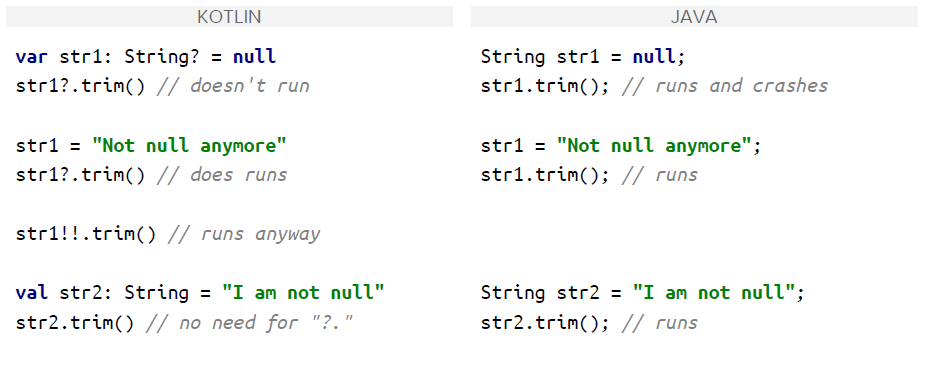
\includegraphics[scale=0.66]{NullSafety.png}
  \caption{{\bfseries Esempio generico degli operatori di Null-Safety}}
  \label{NullSafety}
\end{figure}
